


\chapter{摘要}
LTE 和Wi-Fi链路聚合(简称LWA)和IPSec隧道与LTE WLAN无线电级别集成(LWIP)是3GPP提出的两种方法,以实现5G背景下灵活,通用且可规模化的LTE-WLAN互通性。这些技术可让使用者利用许可和非许可频谱,并允许运营商的公开透明访问核心数据。本文介绍了LWA和LWIP协议的设计细节,并介绍ns-3中的第一个ns-3 LWA和LWIP实现。特别是,这项工作着重于
不同ns-3模块和不同技术协议的适配和并发使用,以支持这些互通方案。

关键词:IEEE 802.11,LTE,无执照LTE,卸载,LWA,LWIP。


%\setcounter{chapter}{1}
%\chapter{一、介绍}
\newpage
\section*{1 介绍}
由于智能手机,平板电脑,可穿戴设备和其他智能移动设备的数量急剧增加,导致对当前和未来无线网络的流量需求有了巨大的增长。根据思科视觉网络指数(VNI)
\cite{index2017global}
,可以知道全球移动到2021年,移动设备产生的数据流量将达到每月48.3 EB,在2016年至2021年之间增长46%。

旨在实现所需的未来容量增长标准化的动机正在3GPP上进行,以使蜂窝移动网络能够在未经许可的2.4和5GHz频谱上运行,这个是Wi-Fi和其他通信系统目前正在使用的频段。迄今为止,有五种不同的方法可将数据从LTE转移到非许可频段:1)LWA 
\cite{access2008and},2)LWIP 
\cite{access2008and},
3)许可辅助访问(LAA)
\cite{afaqui2019implementation},
4)LTE-未经许可(LTEU)
\cite{U-LTE}
,5)MuLTEFire
\cite{alliance2017multefire}
。这些替代方法中的每一种旨在尽可能地满足蜂窝通信的未来增长。然而,在文献中没有根据其实施和性能的可行性对这些进行比较和分析。在这项工作中,我们在ns-3
\cite{Simulator}
中介绍了LWA和LWIP协议的实现细节,以满足上述要求。

ns-3是用于Internet系统的离散事件网络模拟器。它提供了逼真的模型模拟分组数据网络的行为。ns-3通过将运行实际应用程序和网络协议代码的能力与“灵活性”以及在受控网络环境中进行仿真的能力相结合,从而避免重复的工作。ns-3还支持多种模型和协议,例如Wi-Fi,WiMAX,LTE和点对点。提供了使用和修改以实现上述技术的不同ns-3模块的详细信息。LWA和LWIP都已在ns-3.27中实现。

本文的其余部分安排如下。在第2节中,将详细介绍LWA和LWIP机制。第3节和第4节分别描述了LWA和LWIP的实现细节。这两种技术的验证结果在第5节中给出。最后,第6节总结这篇文章。

%\setcounter{chapter}{2}
\newpage
\section*{2 无线局域网互通协议}
\subsection*{2.1 LTE-WLAN无线电聚合}
LWA最早是在3GPP版本13中引入的,它利用Wi-Fi网络在室内的高可用性,将Wi-Fi非许可带宽与许可LTE带宽结合在一起。它在LTE的分组数据融合协议(PDCP)层上有效地集成了LTE和WLAN。LWA旨在实现最佳运行,通过允许LTE和WLAN都承载下行链路流量来确定许可或非许可频段。为了避免Wi-Fi的非对称竞争问题,仅通过LTE承载上行链路。充当用户数据来辅助访问的Wi-Fi AP会连接到LWA基站,因此无需专用网关即可利用LTE核心网络功能。

\begin{figure}[htb]
  \centering
  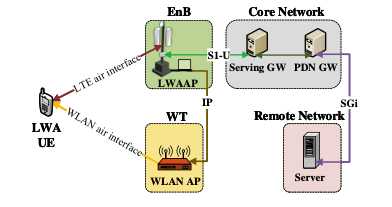
\includegraphics[width=.8\textwidth]{Networ_Architecture_of_LWA.png}
  \caption*{图1:LWA的网络架构}
\end{figure}

LWA的架构包括相关节点B(eNB),支持LWA的Wi-Fi接入点(AP),支持LWA的Wi-Fi站和用户设备(UE)。3GPP LTE的版本13定义了LWA的两个开发场景,即并置和非并置,通过它们,eNB和WLAN实体可以实现连接。在并行的情况下,Wi-Fi 的AP被并置并通过内部回程连接连接到eNB。此部署选项更适合小型小区。对于图1所示的非并置部署,一个称为Xw的可选标准化接口用于通过WLAN终端(WT)逻辑节点(可以是Wi-Fi AP,也可以是WLAN)将WLAN AP连接到eNB。 Wi-Fi控制器)。该接口支持控制(称为Xw-C)和用户(数据)平面(称为Xw-U)。除PDCP服务数据单元(SDU)外,Xw接口还用于“流控制反馈”。的Xw-U接口用于将LWA PDU从eNB传递到WT。的LWA的eNB-WT控制平面信令是通过Xw-C接口信令执行的。它支持以下功能:i)从WT到eNB的WLAN度量的传输,ii)支持UE的LWA(用户平面的建立,管理和控制);iii)Xw管理和错误处理功能。

定义了一个称为LWA自适应协议(LWAAP)的新子层,该子层将数据无线电承载(DRB)ID添加到PDCP帧并将其传输到Wi-Fi接口。这允许将多个承载卸载到Wi-Fi网络。在控制平面中,eNB负责选择要卸载到WLAN的承载,并负责LWA的激活/去激活。但是,版本13没有为接口选择指定任何算法。不管部署方案如何,PDCP帧都是由eNB调度的,其中一些帧用Wi-Fi协议封装并通过Wi-Fi接口传输。LWA还可以配置网络以允许同时使用Wi-Fi和LTE。此过程称为拆分承载,同时使用eNB和Wi-Fi无线电资源。相反,LWA还允许交换承载,它仅利用WLAN无线电资源进行传输。

\begin{figure}[htb]
  \centering
  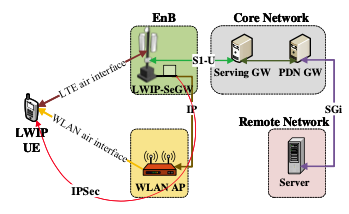
\includegraphics[width=.8\textwidth]{Network_Architecture_of_LWIP.png}
  \caption*{图2:LWA的网络架构}
\end{figure}

在使用拆分承载操作时,UE支持基于3GPP 版本12中引入的用于双连接的重新排序过程,按顺序传送帧。这是通过使用在Windows上运行的重新排序计时器控制的重新排序窗口来完成的,从LTE和Wi-Fi接收的帧通过LWA UE的前述附加PDCP功能被重新排序。在上行链路中,PDCP 的PDU只能通过LTE发送。

\subsection*{2.2 LTE-WLAN无线电级别集成}

3GPP LWIP版本13的基础是由Wi-Fi Boost设置的,它实现了Internet协议(IP)层连接的下行链路交换的第一个实现。LWIP的基本目标是在不做任何重大改动的情况下轻松采用和补充LTE更改WLAN基础架构。图2显示了LWIP方案的网络体系结构。

LWIP中的Tra'c拆分在PDCP层之上执行,并且数据路径绕过所有LTE协议。LWIP聚合方案涉及Internet协议安全性(IPSec)的使用,隧道以通过WLAN基础结构将PDCP SDU数据包从eNB传输到UE。IPSec是一种端到端安全框架(包括用于相互认证的一组协议和算法),它通过扩展帧的IP标头在网络层运行。也就是说,在IPSec隧道模式下,整个IP数据包均受内部和外部IP数据报的保护。内部标头指定通信终结点,而外部IP标头定义加密端点。由于IPSec连接是无需担心WLAN部署,LWIP解决方案支持与LWA(既需要软件又需要添加硬件)相比,传统WLAN部署更容易。

当使用LWIP方案时,在eNB和UE之间交换的无线电资源控制(RRC)和信令消息通过LTE接口承载。为此,指定了一个称为LWIP封装协议(LWIPEP)新协议作为用户平面数据的传输。LWIPEP也用于识别LWIPEP SDU所属的数据承载标识。在PDCP层上方执行流量拆分,并且通向WLAN的数据路径仅通过LWIPEP层(并被PDCP层下方的LTE协议绕过)。LWIPEP协议允许使用为UE配置的IPSec隧道转发不同DRB的帧。重要的是在这里要注意的是,UE不使用任何重排序过程(因为聚合的操作是在PDCP层之上完成的),并且所有LWIP承载数据都被转发了。

由于LWIP对WLAN透明,因此LWA中使用的“ ow控制机制是不适用的。另外,不需要Xw接口和WT节点。但是,由于安全问题,IPSec隧道终止于专用网关,称为安全性网关(SeGW),可以在eNB上部署。

\begin{figure}[htb]
  \centering
  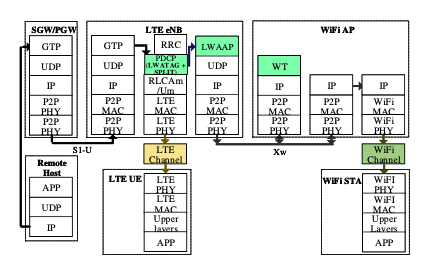
\includegraphics[width=.8\textwidth]{LWA_ns-3_Implementation.png}
  \caption*{图3:LWA ns-3实现}
\end{figure}

eNB负责基于UE测量报告来激活和去激活LWIP操作。该方案的主要缺点是IPSec隧道协议将IPSec标头附加到通过WLAN网络从eNB传输到UE的下行IP数据包。

%\setcounter{chapter}{3}
\newpage
\section*{3 ns-3中LWA的实现}

如第2节强调的,LWA的关键概念是它通过使用eNB中的PDCP层作为汇聚层来启用路由包(即eNB配置处于RRC连接模式的UE使用LTE和WLAN的无线电资源) 。控制平面LTE保持连接,同时数据可以通过eNB和WLAN路由。为了说明该架构是如何在ns-3中进行仿真的,我们参考了图3,该图显示了不同网络设备之间的互连。在这项工作中,我们将研究重点放在版本13中定义的LWA的实现,该版本仅考虑下行链路。

在启动仿真之前,可以命令LTE eNB的PDCP层激活/停用数据卸载。如果LWA被完全激活,则从eNB到UE的数据“停止”,并且该数据被转移到Wi-Fi AP。该过程通过以下方式完成,并通过使用回调函数的事件触发。

\subsection*{3.1 假设}
在我们的实现中,我们做出以下假设:

(1)假设存在非并置的LWA场景,其中LTE网络通过WT连接到已经存在的Wi-Fi网络。

(2)我们假设一个理想的Xw-C接口,其中在沟通和设置上没有错误。

(3)没有考虑流动性模型。

(4)Wi-Fi AP可以容纳普通Wi-Fi站点以及LWA使用的站点。

(5)Wi-Fi站已配置并与AP关联。

\subsection*{3.2 实施细节}
在本节中,我们描述了在ns-3中模拟我们的LWA协议实现过程中发生的动作序列。在本节中,我们将描述发生的操作序列在模拟我们的LWA协议在ns-3中的实现过程中。如图3所示,使用与不同技术(LTE、PointToPoint、Wi-Fi)对应的多个网络组件一起。首先,在远程主机和EPC模型中的UE会尝试遵循直接路径。但是,可以基于部分或全部激活LWA来管理下行链路流量。如果使用完整的LWA,则所有流量都会转发到Wi-Fi网络。而对于部分LWA,某些数据包被允许通过LTE,而其他数据包则被转移到Wi-Fi网络。如图3所示,代表PDCP层上LWA实现的两个主要机制是:LWA Tag和Split。如果激活了部分或全部LWA,则将要传递到Wi-Fi网络的所有数据包都标记为保持自己的身份。在拆分部分中,所有带有LWA标签的帧都将传递到P2P链接以转发到Wi-Fi。所有其他未标记LWA的帧都转发到RLC层。PDCP类中的修改以及LWA中的设计细节ns-3主文件如图4所示。此“ owgraph”提供了详细描述以及随后的“ ns-3中连接LTE和Wi-Fi网络的新添加数据包的数据流”(图3中绿色突出显示的部分与代码添加相对应)。接下来说明如何实现LWA体系结构。

\subsubsection*{3.2.1}
在远程主机上生成数据包,并传输到PDCP层。ns-3中的EPC模型的远程主机为单个UE提供基于IP的服务。OnOff / PacketSink应用程序(模拟IP语音流量)用于通过客户端或服务器配置将UDP数据包突发从远程主机传输到UE。Ipv4StaticRoutingHelper类用于创建静态路由表,以启用远程主机和UE之间通过eNB的连接。生成的数据包的序列号作为标题附加到数据包(称为SeqTsHeader)。

\subsubsection*{3.2.2}
LWA数据流区分。在ns-3中,属性用于组织,记录和修改模型的各个组件使用的默认值。
为了向eNB的PDCP层通知LWA的激活或去激活,因而添加了新的属性。此属性称为lwaactivate。
Add属性将成员变量绑定到公共字符串PDCPDecLwa.在这里重要的是要在属性名称空间中访问变量的值,
该名称空间基于字符串“PDCPDecLwa”和TypeId名称ns3::LtePdcp。该变量用于在仿真开始时激活和禁用LWA连接。
如第2.1节所述,LWA技术还允许部分使用LTE和Wi-Fi技术,以便在UE处按顺序组合数据包。变量可以采用以下值:
i)0-禁用LWA,ii)1-部分LWA(LTE+Wi-Fi)和iii)2-LWA已激活(仅Wi-Fi)。

这些状态还用于模拟LWA的拆分和交换承载操作(1指示拆分承载,而2指示交换承载选项)。

如图4所示,“owgraph”的第一阶段解决了LWA的激活问题。如果未通过设置激活LWA,则将接收到的数据包传递到TransmitPdcpPdu函数,以转发到RLC层。

\subsubsection*{3.2.3}
RBID和LWA激活状态标签。当使用激活部分或全部LWA时,所有数据包在被排队以从LWAAP节点传输之前都被标记有相应的RBID和LWA状态信息。通过从抽象基类ns3::Tag进行子类化来创建两个新标签(
即LWAtag和LCIDtag)。LWAtag包含LWA激活状态,而LCIDtag包含承载的逻辑ID(RBID从LCIDtag派生)。此过程由图4中的“添加LWATag和RBIDTag”实体表示。

\subsubsection*{3.2.4}
LTE PDCP层中的流控制。到达PDCP层的数据包带有变量,该变量被分配了一个值,该值对应于完整的LWA激活,将被标记并排队以通过Wi-Fi基础设施进行传输。
另一方面,如果为变量分配了与部分LWA激活相对应的值,则模运算符用于确定要发送到Wi-Fi AP和eNB的数据包的百分比。
在图中,这由“剩余=PDCPcounter%N“表示4.变量N可以决定拆分百分比,并将其设置为固定值2。因此,当部分LWA被激活时,流量在LTE和Wi-Fi网络之间平均分配。
为了允许在LWA UE上层按顺序传送帧,已经为到达eNB的PDCP层的每个数据包分配了序列号。此数字嵌入在称为SeqTsHeader的12个字节的标头中。序列号和RBID信息可用于在UE处聚合数据。

为了在PDCP层访问数据包,我们利用了依赖于回调和属性系统的ns-3跟踪系统。在PDCP层中添加了一个称为TxPDUtrace的新跟踪源,
该跟踪源可以访问LWA数据包,并用于收集实际传输。为了从eNB的PDCP层提取帧,跟踪接收器功能用于直接对应于回调函数。
即,每当用LWAtag和LCIDtag标记数据包时,
PDCP层上的跟踪回调xPDU函数。
此数据包(包含标头和数据内容)被复制并放入缓冲区以进行传输通过Xw(P2P)链接连接到Wi-Fi网络。这个程序是由图4中的“ Callback LtePDCPTX”框表示。
在这里重要的是提到上述回调函数仅用于标记LWA的帧,并且这些帧不会传递到LTE的eNB的RLC层。

\subsubsection*{3.2.5}
到LWAAP的数据包生成。在3GPP LTE中,典型的传输时间间隔(TTI)设置为1 ms \cite{LTE},该时间间隔是指通过无线电链路进行传输的持续时间。为了及时准确进行从LTE eNB到Wi-Fi AP的帧传输,每隔“ X”个间隔后便会持续观察到缓冲区。该间隔的值保持在上述TTI以下(即,X = 0.1ms)。因此,无论何时将数据包放入缓冲区中,都会立即将其传输到LWAAPnode上的UDP套接字的源。这些过程由图4中的“入队数据包”,“队列为空”和“等待X时间”实体表示。

\subsubsection*{3.2.6}
通过LWAAP制定数据包并传输到Xw链路。如上所述,分组的RBID和序列号是重要的参数,其能够在UE处聚合“ ow”。当将数据包与SeqTsHeader一起复制时,会传递有关序列号的信息。RBID首先从标签中提取lwaactivate信息,然后将其添加为标头以通过Xw接口传输。

如LTE版本13标准中所述,LWAAP实体生成包含RBID身份的LWAAP PDU。为了转发RBID和LWA状态信息,定义了一个名为LwaHeader的新的2字节标头。在下一阶段,数据包被发送到在LWAAPnode上安装的UDP套接字的源。以上图4的LWAAP实体中显示了突出显示的步骤。

\subsubsection*{3.2.7}
数据通过Wi-Fi AP从LWAAPnode转发到Wi-Fi站。从LWAAPnode到Wi-Fi站的数据包的下行链路是通过创建源目标套接字来实现的。假定模拟中的Xw接口是在LWAAPnode和WTnode之间创建的P2P链接。Wi-fi AP也通过P2P链路连接到WT。

LWAAPnode设置为源套接字,Wi-Fi站设置为目标接收器。两个套接字均使用IPv4地址标识。对于套接字之间的同步,两个端口的端口号保持相等。要创建路由数据库并初始化在P2P节点,Wi-Fi AP和Wi-Fi站点之间进行连接的路由表中,使用了Ipv4GlobalRoutingHelper类。

\subsubsection*{3.2.8}
Wi-Fi站的数据包接收。在Wi-Fi站的目标套接字处接收到的数据包包括SeqTsHeader和LwaHeader标头。该信息可以用于在UE的应用层处聚合分组。

借助于表1,我们提供了在ns-3中使用3GPP的LWA标准的LWA实现功能之间的比较。如表中突出显示的那样,3GPP的版本13提供的大多数LWA规范都是在ns-3中实现的。
LWA原为在eNB处进行控制,并在PDCP层执行帧拆分。变量启用了ns-3实现,以支持拆分和交换承载功能。
由于在PDCP层聚合数据的方法的实现工作留作未来的工作,因此在ns-3 LTE UE上未进行任何更改。2如第3.1节所述,假eNB和WT之间存在理想的控制平面(Xw-C)。因此,未考虑WLAN测量,建立,修改和错误处理机制的支持。

\begin{figure}[htb]
  \centering
  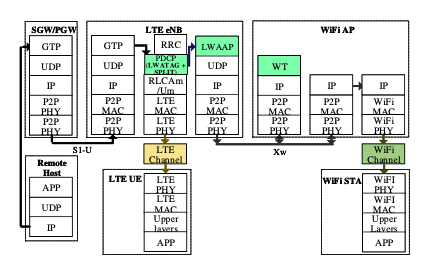
\includegraphics[width=.8\textwidth]{LWA_ns-3_Implementation.png}
  \caption*{图4:LWA实施的流程图}
\end{figure}


\begin{figure}[htb]
  \centering
  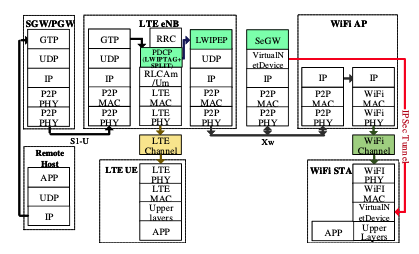
\includegraphics[width=.8\textwidth]{LWIP_ns-3_Implementation.png}
  \caption{图5:LWIP实施的流程图}
\end{figure}

\begin{table}
  \centering
  \caption*{表 1:ns-3 LWA实现和3GPP功能清单}
  \begin{tabular}{|c|c|c|}   %三个c是因为三列,令每列显示在中间显示,也可以是l或r
   \hline         %画一条横线
    属性 & ns-3规则 & 3GPP标准 \\
    \hline 
    eNB控制  & 是  & 是 \\
    \hline 
    连接层  & PDCP  & PDCP \\
    \hline 
    卸载粒度  & 拆分或交换承载  & 拆分或交换承载 \\
    \hline 
    LTE网络升级  & eNB和UE  & 基站 \\
    \hline 
    UE PDCP上的聚合流  &  无 & 是 \\
    \hline 
    LTE中的新网络实体 & LWAAP和Xw-U & LWAAP和Xw \\
    \hline 
    “流量控制”的附加接口  & Xw-U & Xw-U \\
    \hline 
    Xw控制平面接口  & 无 & Xw-C \\
    \hline 
    WT连接建立 & 无 & 是 \\
    \hline 
    Wi-Fi中的新网络节点  & WT & WT \\
    \hline 
    WT连接建立  & 无 & 是 \\
    \hline 
    Wi-Fi中的新网络节点  & WT & WT \\
    \hline 
    WLAN测量 & 无 & 是 \\
    \hline 
    WLAN安全 & 无 & WLAN原生802.1x EAP / AKA \\
    \hline 
    WLAN流量方向 & 下行链接 & 下行链接 \\
    \hline 
\end{tabular}
\end{table}


%\setcounter{chapter}{4}
\newpage
\subsection*{4 ns-3中lwip的实现}
在LWIP中,IPSec隧道用于通过Wi-Fi AP从eNB向UE发送下行链路通信。与LWA相似,LWIP中的UE具有到eNB的RRC连接。与LWA不同,LWIP中的数据包不能同时传输到LTE或WLAN链接。在ns-3中,用于最终用户(包含UE,SGW / PGW和远程主机)的端到端连接的IP网络在EPC模型中不涉及在eNB处使用IP堆栈。为了解决上述问题并获得对PDCP SDU(IP数据包)的访问权限,LWIP协议被设计为遵循3.2节中使用的相同方法,以使LWA在PDCP层提取帧。类似于LWA实现,可以命令LTE eNB的PDCP层激活/去激活数据的卸载。如果激活了LWIP,则完整到UE的LTE停止,数据被转移到Wi-Fi AP。前述过程通过事件驱动的触发技术来完成。在其上创建IP数据包的IPSec隧道被创建在UDP / IP隧道传输的IP数据包上。对于ns-3实现,由于利用了相同的LWA机制,因此使用了Xw接口。事实证明,已实现的Xw-U接口仅负责数据包的传输。


\subsection*{4.1 假设}
在我们的实现中,我们做出以下假设:
(1)假设采用非并置方案,其中LTE网络通过SeGW连接到已经存在的Wi-Fi网络。
(2)我们假设一个理想的Xw-C接口,其中通讯和设置没有错误。
(3)不考虑流动性模型。
(4)Wi-Fi站已配置并与AP关联。
(5)LWIP SeGW与Wi-Fi站之间的LWIP隧道已通过Wi-Fi基础架构建立。
(6)IPSec隧道使用身份验证,但不加密。

\subsection*{4.2 实施细节}
在本节中,我们描述了在ns-3中模拟LWIP协议期间发生的事件顺序。图5表示与不同技术(LTE,PointToPoint,VirtualNetDevice和Wi-Fi)
相对应的多个网络组件一起用于开发LWIP协议。使用VirtualNetDevice创建IP隧道,该VirtualNetDevice使用新的IP标头包装UDP数据包。
首先,从远程主机到UE的任何通信都尝试遵循直接路径。但是,如果要将下行链路流量转发到Wi-Fi网络,则使用安全隧道将数据集中到LWIP UE(即Wi-Fi站)。
PDCP类中的修改以及不同类之间的互连的详细信息在图6中突出显示。该“ owgraph”提供了新的网络节点/模块上的数据包的详细说明和随后的“ ow”信息包,这些新的网络节点/模块被添加为通过IP隧道连接LTE和Wi-Fi网络(图5中突出显示为ns-3的部分)。
接下来说明LWIP体系结构的实现。

\begin{figure}[htb]
  \centering
  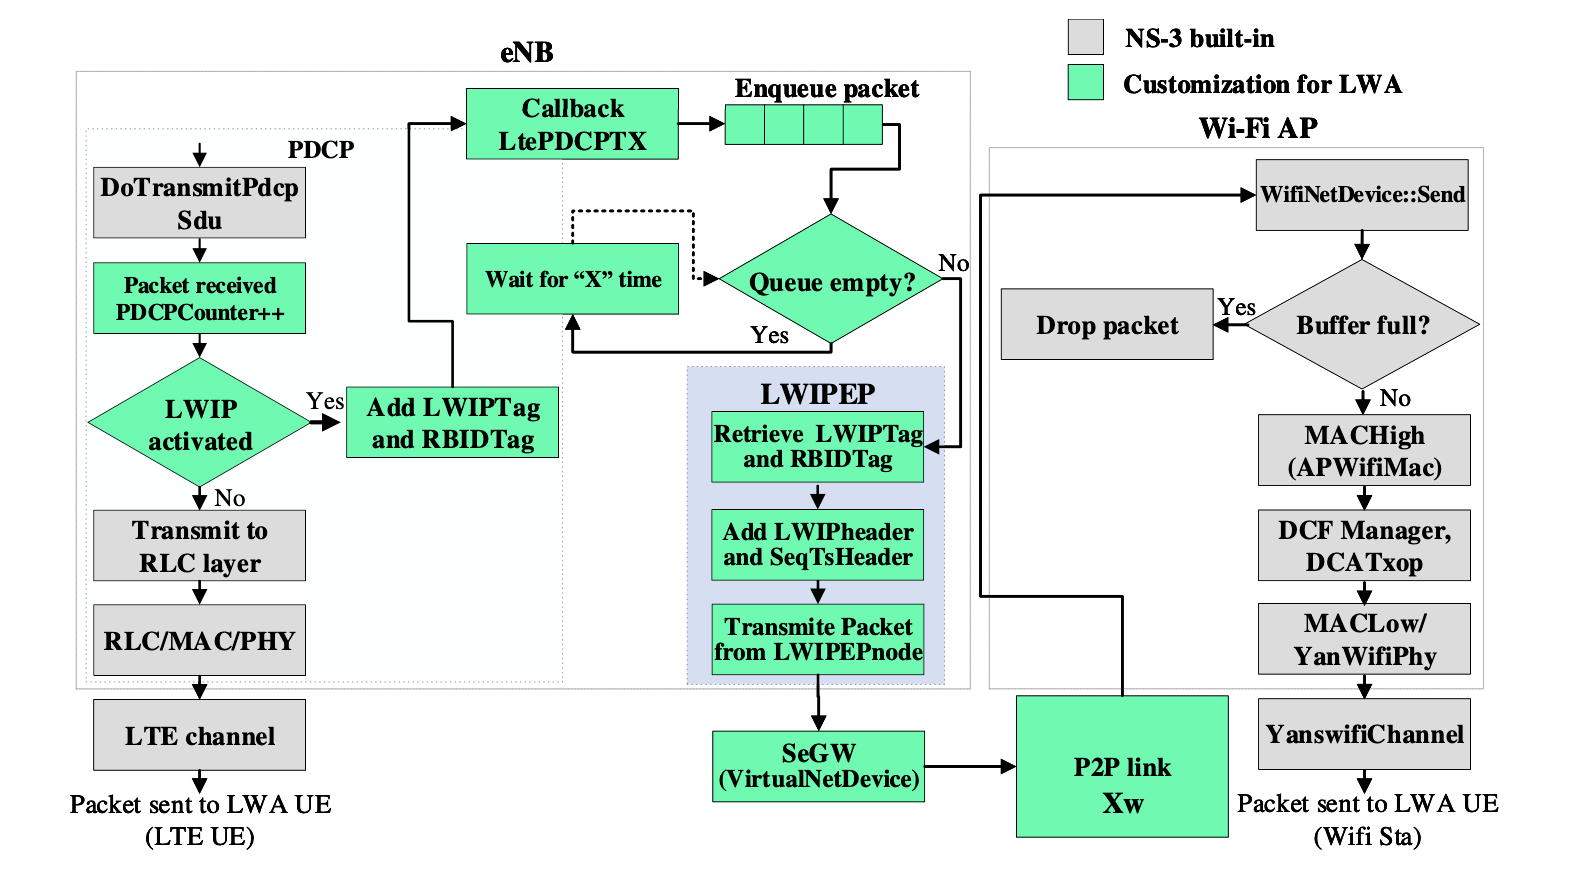
\includegraphics[width=.8\textwidth]{Activity_Diagram_of_LWIP_Implementation.png}
  \caption*{图6:LWIP实施活动图}
\end{figure}


\subsubsection*{4.2.1}
远程主机上的数据包生成,并传输到PDCP层。与LWA实施类似,OnOff/ PacketSink应用程序用于通过客户端/服务器配置将UDP数据包突发从远程主机传输到LTE UE。

\subsubsection*{4.2.2}
LWIP数据流区分。为了将LWIP的激活或去激活通知给eNB的PDCP层,添加了新的属性。
此属性称为lwipactivate,
与用于访问基础成员变量的机制相关联,
该成员变量用于激活和停用LWIP连接。
i)0-禁用LWIP,并且ii)1-LWIP被激活。

在模拟开始时,Config :: SetDefault方法用于覆盖PDCPDecLwip属性的初始(默认)值。
如图6所示,“owgraph”的第一阶段用于做出有关LWIP激活的决定。如果未通过设置激活LWIP,则将接收到的数据包传递到TransmitPdcpPdu函数,以转发到RLC层。

\subsubsection*{4.2.3}
RBID和LWA激活状态标签。与LWA相似,当为变量分配一个与LWIP激活相对应的值时,所有数据包在被排队以从LWIPEP节点传输之前都被标记有相应的RBID和LWIP状态信息。为LWA定义的LCIDtag被重用。怎么样曾经,对于LWIP状态,定义了一个新标签(称为LWIPTag)。这在图10中显示为实体“添加LWIPTag和RBIDTag”。

LTE PDCP层中的流控制。到达PDCP层的数据包带有变量,该变量被分配了一个与LWIP激活的值相对应的数据包,将被标记并排队以通过Wi-Fi基础设施进行传输。为了允许在LWA UE上层按顺序传送帧,已经为到达eNB的PDCP层的每个数据包分配了序列号。此数字嵌入在12个字节的SeqTsHeader中。为了从PDCP层提取带有LWIP标签的帧,使用了第3.2.4节中描述的相同方法。

\subsubsection*{4.2.4}
LTE 
PDCP层中的流控制。到达PDCP层的数据包带有变量,该变量被分配了一个与LWIP激活的值相对应的数据包,将被标记并排队以通过Wi-Fi基础设施进行传输。为了允许在LWA UE上层按顺序传送帧,已经为到达eNB的PDCP层的每个数据包分配了序列号。此数字嵌入在12个字节的SeqTsHeader中。为了从PDCP层提取带有LWIP标签的帧,使用了第3.2.4节中描述的相同方法。

\subsubsection*{4.2.5}
到LWIPEP实体的数据包生成。3.2.5节中描述的过程用于将数据包传输到LWIPEPnode。

\subsubsection*{4.2.6}
由LWIPEP制定数据包并传输到SeGW链路。
如第2.2节所述,LWIPEP模块的职责是生成用户纯数据以及承载者标识。类似于LWA,首先从标记中提取RBID和lwip激活信息,然后将其作为标头添加到要通过Xw接口发送的数据包中。
定义了一个名为LwipHeader的新的2字节标头,其中包含lwip激活状态和承载ID信息。此阶段由图6中的LWIPEP实体表示。

在下一阶段,数据包从LWIPEPnode传输到SeGW,以通过IPSec隧道传输。

\subsubsection*{4.2.7}
通过IP隧道将数据从SeGW转发到Wi-Fi站。为了创建IP隧道,在SeGW链接上安装了额外的虚拟接口,并在Wi-Fi站上安装了虚拟接口(即,在P2P链接上安装了新地址设置为11.0.0.1的接口,并安装了地址为11.0.0.254的接口)通过Wi-Fi站)。因此,“数据包的流量将在11.0.0.x之间(即隧道)而不是实际的IP地址(P2P和192.168.xy为10.0.xy用于Wi-Fi网络)。SeGW上VirtualNetDevice的使用代表了与外部Wi-Fi网络的联系点。这是启动安全IPSec隧道的地方。创建一个使用回调函数在VirtualNetDevice上创建虚拟UDP源套接字和目标套接字的隧道类。这些套接字用于将IP封装的LWIP数据包从SeGW传输到Wi-Fi站。为LWA定义的Xw接口被重用于提供SeGW和Wi-Fi AP之间的连接。


\subsubsection*{4.2.8}
Wi-Fi站的数据包接收。在Wi-Fi站点的目的地接收到的数据包包括SeqTsHeader和LwipHeader标头。该信息可以用于在UE的应用层处聚合分组。


因此,详细的WLAN测量,支持建立,修改和错误处理机制都没有被考虑。尽管可以将LWIP配置为通过WLAN传输上行链路和下行链路数据,但我们将研究重点放在了实现上,尤其是下行链路通信。

\newpage
\subsection*{5 绩效评估}
在本节中,我们描述评估方案的定义和结果的收集。我们评估了通过使用LWA和LWIP所获得的总容量,以及它们如何在效率和与附近具有Wi-Fi干扰网络相关的不同影响方面进行比较。表3列出了所使用的参数,对于LWA和LWIP Wi-Fi传输,我们考虑了没有MIMO和聚合。模拟运行100秒,已重复10次。我们使用恒定比特率(CBR)UDP源.


\begin{table}
  \centering
  \caption*{表 2:ns-3 LWIP实现3GPP功能清单}
  \begin{tabular}{|c|c|c|}   %三个c是因为三列,令每列显示在中间显示,也可以是l或r
   \hline         %画一条横线
    属性 & ns-3 LWIP & 3GPP标准LWIP \\
    \hline 
    eNB控制  & 是  & 是 \\
    \hline 
    连接层  & PDCP  & IP (PDCP SDU)P \\
    \hline 
    卸载粒度  & 交换承载  & 交换承载 \\
    \hline 
    LTE网络升级  & 基站  & 基站 \\
    \hline 
    UE PDCP上的聚合流  &  无 & 是 \\
    \hline 
    LTE中的新网络实体 & LWIPEP和SeGW & LWIPEP和SeGW \\
    \hline 
    Wi-Fi中的新网络节点  & 无 & 无 \\
    \hline 
    WLAN测量  & 无 & 是 \\
    \hline 
    WLAN安全 & 无 & WLAN原生802.1x EAP / AKA \\
    \hline 
    WLAN流量方向 & 下行链接 & W下行加上上行 \\
    \hline 
\end{tabular}
\end{table}

我们首先比较未许可频谱中LWA和LWIP的效率。为此,我们模拟了1个eNB,1个Wi-Fi AP,1个Wi-Fi STA和1个UE,同时eNB生成了朝向UE的下行链路流量。为了评估网络效率,我们LTE和Wi-Fi通道都饱和。也就是说,我们使确保始终有一个要由eNB和Wi-Fi AP传输的数据包。这样,我们可以比较LWA和LWIP的最大容量。在没有其他网络干扰的情况下,由于IPSec隧道的额外报头会减少LWIP可以在每个站点传输的有效信息,因此我们希望LWIP能够以比LWA更低的程度增强LTE容量。Wi-Fi传输尝试。结果绘制在图7中,其中显示了未激活LWA和LWIP时的LTE吞吐量,以及通过使用LTE以及具有可变数据包大小的LWA和LWIP获得的聚合容量。请注意,由于此处假设处于饱和条件,因此使用部分或全部LWA不会对吞吐量结果产生任何影响。因此,我们有选择仅显示完整的LWA结果。

\begin{table}
  \centering
  \caption*{表 3:仿真参数}
  \begin{tabular}{|c|c|c|c|}   %三个c是因为三列,令每列显示在中间显示,也可以是l或r
   \hline         %画一条横线
    Wi-Fi参数 & 值 & 升参数 & 28\\
    \hline 
    发射功率 & 30 dBm & 发射功率 & 30 dBm\\
    \hline 
    带宽 & 20兆赫 & 升参数 & 28\\
    \hline 
    Wi-Fi参数 & 值 & 传输带宽配置[NRB] & 25(5 MHz)\\
    \hline 
    RTS/CTS & 否 & 噪声系数 & 5\\
    \hline 
\end{tabular}
\end{table}


从图7中可以看出,对于所考虑的参数,LWA和LWIP的使用可以显着提高总容量。请注意,我们使用了IEEE 802.11ac参数,并且获得的Wi-Fi吞吐量可以高达78 Mbps。正如我们之前介绍的,我们可以观察到,使用LWIP会导致吞吐量略低于LWA。这是由于IPSec隧道的额外标头所致。我们可以在以及增加数据包大小的效果(每个数据包传输的有效数据)。在Wi-Fi结果中增加数据包大小和每次通道尝试传输更多数据时,吞吐量会更高,通过补偿开销(无论是标头还是通道访问效率)(例如由于DIFS,SIFS和backo )插槽而导致的空通道持续时间)。从图中可以看出,这种趋势的综合效果(随着数据包大小的增加,吞吐量增加)和更高的LWIP与LWA相比,效率低下。请注意,对于较小的数据包大小,由于开销引起的LWIP较高的效率更加明显。对于更长的数据包大小,随着通道访问变得更加有效,在LWIP中引入的额外增加的开销可以忽略不计。

\begin{figure}[htb]
  \centering
  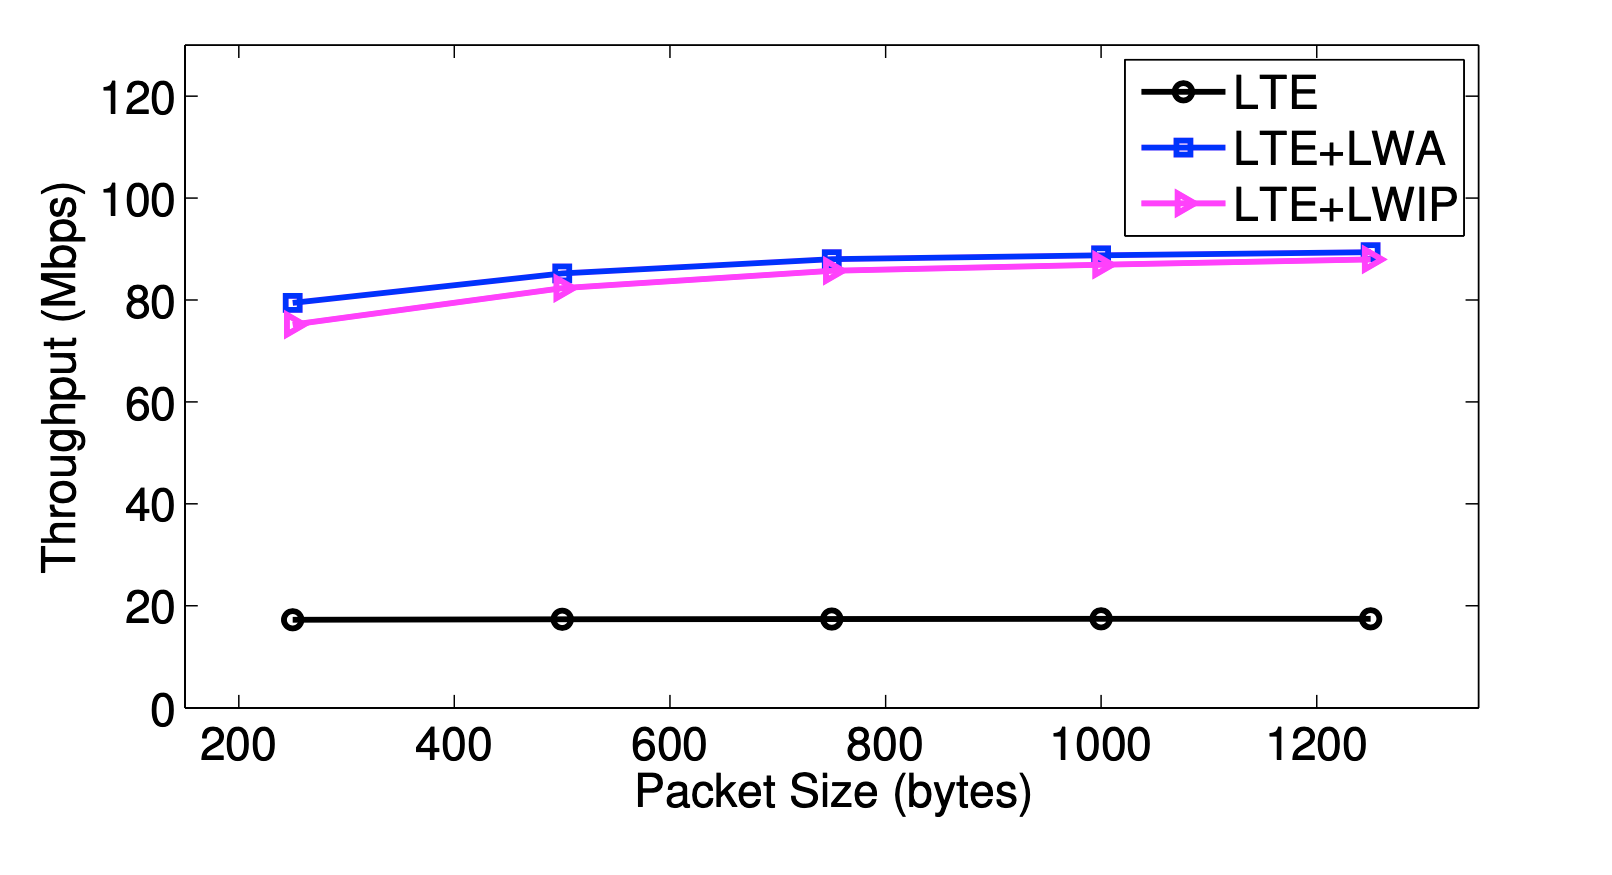
\includegraphics[width=.8\textwidth]{LTE_Aggregated_Capacity_using_LWA_and_LWIP.png}
  \caption*{图7:使用LWA和LWIP的LTE聚合容量}
\end{figure}

现在,我们评估具有Wi-Fi网络干扰LWA和LWIP链路的影响,并分析Wi-Fi网络中上行链路传输数量增加的影响。因此,有效评估LWA和LWIP在竞争下的表现。图8显示了LTE链路的吞吐量以及LWA连接(现在不再与LTE进行汇总,以便更好地与Wi-Fi比较)所实现的吞吐量Wi-Fi干扰网络中实现的吞吐量。现在,发射功率已设置为15 dBm,Wi-Fi和LTE的数据包大小均已设置为500字节,载波侦听阈值已设置为-72 dBm。仿真时间已设置为10 s

我们可以在图8中观察到,随着上行链路Wi-Fi发射机数量的增加,LWA和LWIP的吞吐量会下降。这是由于Wi-Fi的信道访问可为每个设备提供公平性。我们看不到所有设备(2、4和6个Wi-Fi发射器以及LWA / LWIP AP)之间的资源分配比例,由于默认情况下ns-3优先处理AP通道访问。但是,即使使用更高的优先级,我们也可以在图中看到,随着来自Wi-Fi网络的争用,LWA和LWIP吞吐量会大大降低。同样有趣的效果是,随着Wi-Fi干扰源数量的增加,由于必须传输额外的报头而导致的LWIP的效率变得微不足道。我们认为,这是由于与争用导致的信道访问效率低下相比,这种额外开销现在可以忽略不计。还值得注意的是,即使将LTE带宽设置为5 MHz,将Wi-Fi侧的带宽设置为20 MHz,通过LWA和LWIP连接获得的吞吐能力也比LTE链路的吞吐能力小。但现在需要与共存的Wi-Fi网络共享

\begin{figure}[htb]
  \centering
  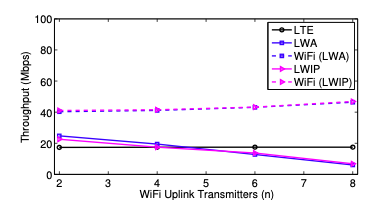
\includegraphics[width=.8\textwidth]{Throughput_Achieved_in_the_LTE_and_LWA_Link_when_a_Wi-Fi_Interferer_Network_is_Placed_in_the_Vicinity.png}
  \caption*{图8:将Wi-Fi干扰网络放置在附近时,LTE和LWA链路中实现的吞吐量}
\end{figure}

在下文中,我们评估了具有Wi-Fi网络干扰源的影响,并通过增加两个网络(Wi-Fi和LWA链路)之间的距离以及通过增加两个网络之间的距离来分析干扰的影响如何变化。 Wi-Fi干扰网络和LWA连接的传输功率。图9显示了LTE链路的吞吐量以及通过LWA连接实现的吞吐量(现在不再与LTE集成在一起,以更好地实现与Wi-Fi进行比较),以及在Wi-Fi干扰网络中实现的汇总吞吐量。Wi-Fi发射机的数量(仅在上行链路中)被认为等于n = 2和n = 3。现在,发射功率设置为15 dBm,LWA链路和Wi-Fi网络的数据包大小设置为1000字节,载波侦听阈值设置为-72 dBm。在5.19 GHz Wi-Fi频带中使用三个对数距离传播路径损耗模型(路径损耗指数为α1= 2,α2=α3= 3.5)。仅显示LWA的结果,因为LWIP的性能类似于图8。

从图9中可以看出,当两个网络靠近时,由于它们现在共享信道资源并创建竞争,因此实现的吞吐量会大大降低。只要我们增加它们之间的距离,吞吐量就会提高,直到它们不再相互干扰为止。从小距离可以看出,当Wi-Fi干扰源与2个节点而不是3个节点竞争时,通过LWA达到的吞吐量更高。同样,n = 2时,LWA链路的吞吐量大约是Wi-Fi网络实现的吞吐量的一半。值得注意的是,通过增加LWA接收器将获得相反的效果。但是,我们没有观察到完全比例除法由于LWA设备是AP,并且某些信道访问参数默认在ns-3中优先于AP传输,因此根据网络用户数分配资源。

\begin{figure}[htb]
  \centering
  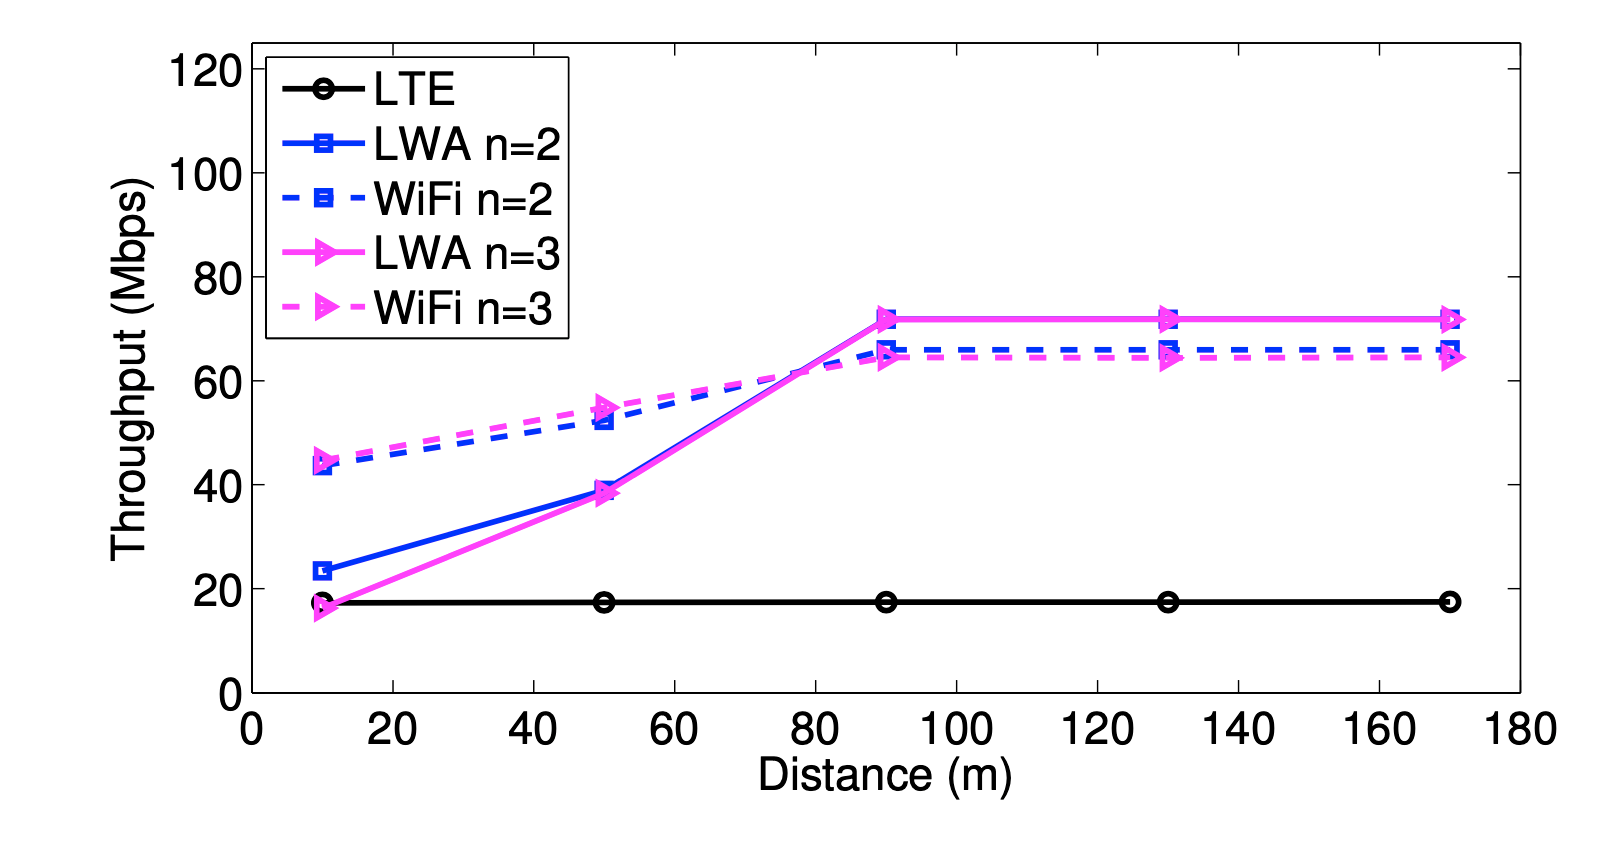
\includegraphics[width=.8\textwidth]{Throughput_Achieved_in_the_LTE_and_LWA_Link_when_a_Wi-Fi_Interferer_Network_is_Placed_in_the_Vicinity2.png}
  \caption*{图9:将Wi-Fi干扰网络放置在附近时,LTE和LWA链路中实现的吞吐量}
\end{figure}

这就是LWA链路传输在此结果中以某种方式受益于与Wi-Fi共享的无执照频谱的原因。有趣的是,我们也可以从该图中看到,即使Wi-Fi信道带宽被认为等于20 MHz,而LTE被设置为LTE,现在吞吐量也可以与LTE链路中的吞吐量相媲美。这些仿真为5 MHz。

\newpage
\section*{6 结论}
在本文中,我们介绍了3GPP在版本13中提出的LTE-WLAN卸载技术(即LWA和LWIP)实现的设计细节。我们提供了这两种技术的详细信息,并提供了实现的不同方面的分步说明,并通过仿真结果对其进行了验证。首先,我们分析了饱和条件下LWA和LWIP实施的效率。结果表明,在没有干扰的情况下,LTE-WLAN互通方案的总容量将大大增加。但是,由于IPsec隧道开销,发现LWIP的效率较低。接下来,观察到来自相邻Wi-Fi小区的干扰对主要WLAN网络(支持LWA / LWIP)的影响。重要的结果是,对于友好操作,应选择较少的主单元干扰附近的电台。未来的工作包括将ns-3中的LAA与我们已实现的LWA / LWIP技术进行比较。

\chapter{致谢}
% \section*{致谢}
这项工作已得到欧洲地平线2020计划根据赠款协议732174(ORCA项目,UP-ORCA EXT3)的部分支持,并得到了欧洲区域发展基金TEC2015-71303-R的资助(MINECO / FEDER)的部分支持。


